\section{Introduction}

The deployment of deep neural networks in safety-critical domains such as autonomous driving and medical diagnosis has necessitated rigorous verification of their properties. One of the most critical properties is \textit{local robustness}, which certifies that a network's prediction remains invariant under small perturbations to the input. \texttt{DeepPoly}\cite{singh_gehr_püschel_vechev_2019} provides us with a clear method to certify output bounds for a given neural network. Let us consider the situation where we are given a trained neural network $f(\mathbf{I})$ on some set $\mathbf{I}$. Then, under some input $x_0 \in \I$ and perturbation $\epsilon$, we need to verify that the output of $f$ still satisfies the same result i.e. we want to verify that the neural network is invariant to a $\epsilon$ perturbation of the input. This can formally be represented as:
\begin{align*}
    \forall x \in \mathbb{B}_\infty(x_0, \epsilon): \quad \text{argmax}(f(x)) = \text{argmax}(f(x_0))
\end{align*}
where, $\mathbb{B}_{\infty}$ is a ball of $\epsilon$ radius around the input provided by its $\Ll_{\infty}$ norm as shown in Fig~\ref{fig:robustness_verification}. This is critical in a lot of scenarios as with many supervised learning problems, it is infeasible to verify the output of a neural network against all possible test sets. We want to formally prove that the model is invariant to these input changes.

\begin{figure}[ht!]
    \centering
    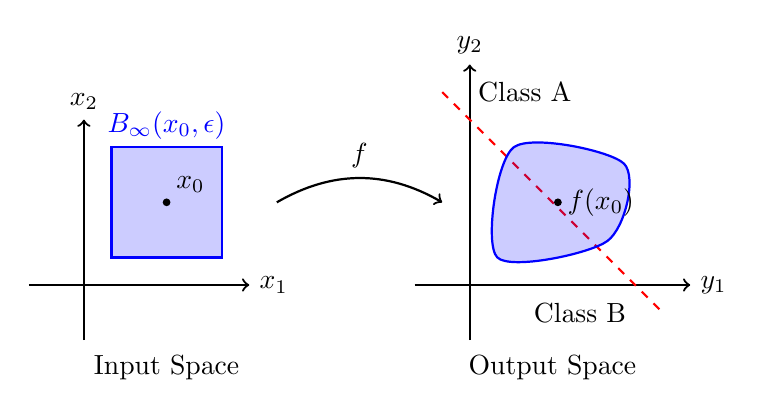
\begin{tikzpicture}[scale=0.7]
        \draw[thick, ->] (-1,0) -- (3,0) node[right] {$x_1$};
        \draw[thick, ->] (0,-1) -- (0,3) node[above] {$x_2$};
        \draw[blue, thick] (0.5, 0.5) rectangle (2.5, 2.5);
        \fill[blue, opacity=0.2] (0.5, 0.5) rectangle (2.5, 2.5);
        \fill[black] (1.5, 1.5) circle (2pt) node[above right] {$x_0$};
        \node[blue] at (1.5, 2.9) {$\mathbb{B}_\infty(x_0, \epsilon)$};
        \node at (1.5, -1.5) {Input Space};

        \draw[->, thick, bend left] (3.5, 1.5) to node[midway, above] {$f$} (6.5, 1.5);
        \begin{scope}[shift={(7,0)}]
            \draw[thick, ->] (-1,0) -- (4,0) node[right] {$y_1$};
            \draw[thick, ->] (0,-1) -- (0,4) node[above] {$y_2$};
            \draw[red, thick, dashed] (-0.5, 3.5) -- (3.5, -0.5);
            \node[red, rotate=-45] at (2.8, 0.8) {};
            \draw[blue, thick] plot [smooth cycle] coordinates {(0.5,0.5) (2.5,0.8) (2.8,2.2) (0.8,2.5)};
            \fill[blue, opacity=0.2] plot [smooth cycle] coordinates {(0.5,0.5) (2.5,0.8) (2.8,2.2) (0.8,2.5)};
            \fill[black] (1.6, 1.5) circle (2pt) node[right] {$f(x_0)$};
            \node at (1.5, -1.5) {Output Space};
            \node at (1.0, 3.5) {Class A};
            \node at (2.0, -0.5) {Class B};
        \end{scope}
    \end{tikzpicture}
    \caption{The input region $\mathbb{B}_\infty(x_0, \epsilon)$ (left) is mapped by the neural network $f$ to a region in the output space (right). Verification succeeds if the entire mapped region lies within the decision boundary (dotted red) of the correct class (Class A). This illustrates the robustness verification problem.}
    \label{fig:robustness_verification}
\end{figure}

The earliest solutions that attempted to solve this problem are end-to-end/complete verification solutions.~\cite{katz2017reluplex} introduced a tool called \texttt{Reluplex}, which is a solver based on SMT that combined the Simplex algorithm with ReLU activation functions to exactly verify small neural networks. Later,~\cite{tjeng2019evaluating} used Mixed Integer Linear Programming (\texttt{MILP}) to write the problem as a commercial solution that exactly calculates robustness bounds. Although these solutions are sound and complete, they are NP-complete problems, known to not scale with the size of modern neural networks which are deployed in safety-critical applications.

For overcoming the scalability issue, Abstract Interpretation~\cite{cousot_radhia_cousot_1977} and later for neural networks~\cite{Gehr2018AI2SA} has been adopted, which is less complete but more efficient because it over-approximates how the network behaves.~\cite{Weng2018TowardsFC} introduced a way to quickly compute robustness certificates with a linear bound propagation approach. The \texttt{DeepPoly}\cite{singh_gehr_püschel_vechev_2019} approach pushed the boundaries even further by combining floating-point polyhedra with intervals, which, thanks to linearization, managed non-linearities such as Sigmoid and Tanh activations. More recent contributions, such as ~\cite{NEURIPS2018_f2f44698}

In our research, we ask the following question:
\begin{quote}
    \textit{Can we continue to prove robustness properties of a neural network by leveraging the properties of dual numbers and information about the gradients?}
\end{quote}

We proceed with the foundation built on the \textit{Abstract Dual Domain}. Our research is based on the theory of forward-mode automatic differentiation, which uses a concept called \textit{dual numbers}\cite{griewank2008evaluating}. We aim to analyze the sensitivity of the neural network to changes in the input, which can potentially provide a tighter bound on certain verification problems. In summary, our contributions are:
\begin{itemize}
    \renewcommand{\labelitemi}{\tiny$\square$}
    \item \textit{Algorithmic Realization of Abstract Duals:} We implement a sound abstract domain for dual numbers that explicitly handles curvature error for non-linear activations using Taylor expansion bounds.
    \item \textit{Gradient-Based Verification Logic:} We formulate a sufficient condition for local robustness based on global Lipschitz bounds derived from the abstract gradient.
    \item \textit{Gradient Instability Metric:} We introduce a diagnostic metric, $\mathcal{I}_{unstable}$, which detects zero-crossings in gradient intervals and serves as a predictor for the breakdown of local linearity.
    \item \textit{Empirical Analysis:} We evaluate our method against \texttt{DeepPoly}, identifying a specific ``shallow and smooth'' regime where global gradient bounds outperform layer-wise relational abstractions.
\end{itemize}